
\chapter{Reference Model Construction}
%%%%%%%%%%

This chapter conceptions the process reference model and is central part of this thesis. In order to discuss particular processes, the framework itself needs to be discussed. What follows is the discussion of processes, which puts special emphasis on design decisions, \viz \textit{how} to model certain aspects with constructs of the language icebricks. 

	%%%%%%%%%%
	deloitte W14: managing change dispute:::: innovation und so... wichtig für begründung des frameworks
	\section{Process Framework}
	
	\citeauthor{Meise2001} defines a framework as \enquote{an ordering relevant elements and relationships on a high level of abstraction. [...] Purpose is to give an overview about an original and to support structuring of elements and relationships on lower detail levels} \citep[\p{62}]{Meise2001}. Drawing further on his work, which especially targets framework design in process-oriented organizations, the proposed procedure for construction is adopted (\Fig \ref{fig:meise}). Differences to his approach arise, as the reference model should display as as-is state of the domain and does not follow goals of reorganization set by a specific company. Therefore, the \textit{organization} represents a fictive BPO provider in CRM in the following, which captures generic aspects of the domain. The construction is split into two components. The structural part first encompasses strategic and fundamental reflections, while the graphical component transfers these into a visual form that supports communication.

	\begin{figure}[caption={procedure for framework construction}, label={fig:meise}]
		{	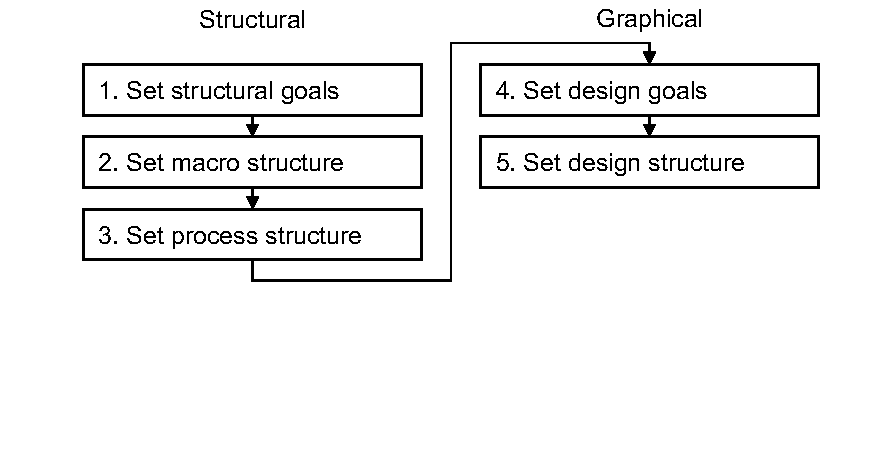
\includegraphics[width=.8\textwidth]{figures/framework-meise.pdf}}
		\hspace{6.2cm}	SOURCE:  adapted from \citep[\p{122}]{Meise2001}
	\end{figure} 
	
	\subsubsection{Ad 1. Set structural goals}
	
	Modeling is no end in itself and different purposes require different models. Theoretically speaking, purpose of this research is to create an artifact that generates utility and tackles a problem in the real-world.  Previously identified problems (\ref{sec:proide}) lead to objectives (\ref{sec:solobj}) which are to be faced with the process reference model in general and its framework in particular. The existence of general (organizational) and stakeholder-related objectives requires the framework to bring together both ends, as it is the basis of the model. 
	
	\begin{table}[caption={Solution Objectives}, label={tab:solobj}]
		\centering
		\begin{tabular}{l p{13.3cm}}

			\textbf{No. }&\textbf{ Solution Objective}
			 \\ \hline
			\textbf{1 }                        & Construction of a generic reference model that covers distinguishing processes for BPO-providers in CRM on concept level.                                                    \\ \hline
			\textbf{2}                         & The reference model can be applied for use at Arvato CRM.                                                                                                                    \\ \hline
			\textbf{3 }                        & The construction,process is well-documented, makes use of empirical research by induction, which is enriched by deduction from \acrshort{BPO} and \acrshort{CRM} theory. \\ \hline
			\textbf{4}                         & A syntactic and semantic formalized process modeling language is used, that is transferable to other languages.                                                              \\ \hline
			\textbf{5}                         & The model can be used as a statement of competence for sales activities towards clients.                                                                                     \\ \hline
			\textbf{6}                         & The model holds a process representation, which supports a common understanding across client businesses.                                                                    \\ \hline
			\textbf{7}                         & The model is able to represent an omni-channel environment.                                                                                                                 
		\end{tabular}
	\end{table}

	
	
	\subsubsection{Ad 2. Set macro structure}
	
	A framework, as a strategic tool, incorporates concepts of strategy. One can name two perspectives, namely a market- or resource-based view of strategy, which are directed externally or internally, respectively. They are not independently of each other, but their interplay is seen as an important factor in strategic decision making. \cite{becker2004handelsinformationssysteme} note, that standardization in keeping with reference model application has contra-productive effects on strategic competitive advantages. This argument is true, when the reference model is used as a application model. The application of the reference should incorporate strategic characteristics of the company, which implies that this reference model framework can only capture a strategic orientation as perceived useful by the author. 
	
	The market-based view follow the structure-conduct-performance paradigm, that explains success of a company through external factors in the industry. \cite{porter1980} formulated the so called five-forces model, which describes bargaining power of suppliers (1), threat of substitutes (2), bargaining power of buyers (3), threats of new entrants (4) and industry rivalry (5) as determinants of competition. Applying these two the BPO domain, a trivial substitute for outsourced services is the return of services inside the parent organization. Further, the substitution of customer services through automation may render outsourcing obsolete. The bargaining power of suppliers and buyers can be loosely mapped to clients and customers. While clients as suppliers clearly influence the provider directly, customers show less of this influence on the outsourcing provider. As the provider takes an intermediate position between client and customer (\cf \Fig \ref{fig:bpochain}), their acting is always in connection with the client. However, an assessment of outsourced service quality puts pressure originating from the customer on the provider, which in turn will also be judged by the client. The entry of new players on the market (4) can be tackled by barriers, that go back to competitive advantages of differentiation or cost-leadership. While the latter is especially causing fierce competition in low-wage regions that realize offshore-outsourcing, outsourcing players in CRM that feature more profound services, lean towards a differentiation strategy. This can also be stated for Arvato. Lastly, industry rivalry among players in the BPO CRM market is also influenced by the aforementioned generic strategies, to position established companies. A framework adopts market-based aspects through accounting for markets or segments therein. These are accompanied by business units or processes that relate to this external environment. 
	
	The resource-based view of strategy analyzes internal strengths and weaknesses. Resources are bundled to form capabilities and should be rare, inimitable, create value and be non-substitutable. Due to asymmetries of resources, competitive advantages are enabled. The identification of capabilities of CRM BPO providers (\cf \ref{sec:bpocrmis}: operational and business development capabilities) can only be done on a generic level for the reference model. Application necessitates specifying the framework to conform to company-specific capabilities. The operational capability should reflect the operational process component in CRM (\cf \ref{crmprocessfr}), and service delivery from the outsourcing side (\cf \ref{app:provproc}). Business development, \ie understanding and addressing client needs, misses a pendant in an isolated CRM view, but can be put in relation to delivery management in the outsourcing model. 
	
	Putting both views together emphasizes the client and customer market environment and two capabilities, that relate to these markets. Towards the client side, providers are criticized by clients for being too reactive instead of proactive (49\%), delivering poor service quality (48\%) and lack of innovation (37\%) \citep{deloitte2014outsourcing}. While the first point of criticism addresses the client relationship, the other two are directed towards the service itself. Looking at the constituents of \acrshort{CRM}, the people, process, technology split draws a line to the resource-based view, as these three resources need to be developed and captured to enable superior service provision for clients. Apart from the  \acrshort{CRM} view, these three also have their own meaning in \acrshort{BPO}. The importance of processes in  \acrshort{BPO} is obvious. The people component can be interpreted here as the provision of manpower and their training for services; (information) technology as an enabler of outsourcing (\cf \ref{sec:bpo}) . 
	
		
	\subsubsection{Ad 3. Set process structure}
	
	Given that the model shows processes, the structural split of people, processes and technology is hardly meaningful, as two aspects of  \acrshort{CRM} or \acrshort{BPO} would be left out. Drawing from the BPO chain and the identified stakeholders enables another categorization that leaves room for design choices, while capturing generic aspects of business processes within \acrshort{BPO}. As \acrshort{BPO} is the framing construct and  \acrshort{CRM} one use of it, this order is to be prioritized. The following briefly describes business processes, that are detailed in the remainder of this chapter.
	
	
	\begin{figure}[caption={BPO chain provider scope with stakeholders}, label={fig:bpochainscope}]
		{	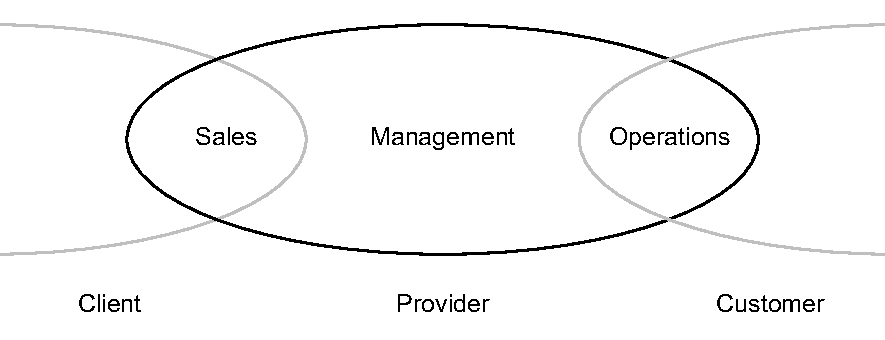
\includegraphics[width=.8\textwidth]{figures/chain2.pdf}}
	\end{figure} 
	
	\textit{Sales}-related business processes cover processes that have touchpoints with the client. These take place along a lifecycle, which starts with initial contact between provider and client, and hopefully advances through creation of an outsourcing contract. For this agreement, the \acrshort{BPO} provider places its products (\ie, service blueprints) in the clients requirements profile, so create solutions for identified problems. Also, the implementation and setup of the outsourced business must take place. After everything is set up, the client relationship is maintained under the umbrella of account management. 
	
	\textit{Management}-related business processes bring together resources in the provider organization, so that the operations and business development capability are realized. Regarding the latter, it is important to have a products in place, which can be implemented as service solutions for clients.  \citep{schewe2007} names this delivery management, but explicitly refers to its similarities with product development. In addition to the development, the management of existing products inside a product portfolio becomes important. The operations capability can be addressed by processes, that enable economies of scale. Benefits through economies of scope are a question of offered services and not processes. Economies of scale are realized by the increased output of services across client businesses, which in turn necessitates alignment in these services so that their output can be counted \enquote{together}. This alignment is facilitated through a product-view of services and their underlying portfolio in the organization. In addition, people in the provider organization need to be trained  in order to excel in the role of \acrshort{CSR}. Their career path can be seen from a process perspective, so that a strong relationship is established with their employer. This aspect shall be called People Lifecycle Management. Lastly, management of the workforce, especially scheduling, becomes critical in a business like customer service. The assurance of the right capacity at the right time to meet fluctuating demand with little waiting time is expected from the client. Therefore, efficient techniques to manage the complexity of multiple channels, different demand patterns and differently skilled \acrshort{CSR}s are necessary. This is encapsulated in the process of workforce management. 
	
	\textit{Operations}-related business processes target the service delivery in the words of \citeauthor{schewe2007}. The processing of transactions with customers is in focus, which can be on numerous channels. A transaction in this case is a conversation, so that theories of communication \citep{shannon1949} may be used here.  A message is sent from a sender to a receiver through a medium. In case of customer service, both the customer or the \acrshort{CSR} can start a conversation, that has a subject which relates to the client in some way. Reasons for contact may be separated by being related to a previous transaction. This transaction might be a purchase of a client's good or service. The communication channel increasingly varies and is no reasonable split, as in an omni-channel environment a seamless experience across channels is intended. Hence, the processes should be similar on a high level of abstraction. 
	
	Communication can be asynchronous (\eg, e-mail) or synchronous(\eg, voice), which puts emphasis on temporal differences in the conversation. While the employed process definition encompasses the \enquote{time-logical sequence of activities}, the value(\viz time between activities) does not impact the process logic itself, as this is a question of succession. General steps in inquiry handling from a business perspective will be similar independent of the (a)synchronous case. What becomes important from a business perspective is the question who initiates the customer contact. A communication triggered by the customer (incoming) follows demand patterns that are inferred from historic data, while better planning of \acrshort{CSR} opened contacts (outgoing) is possible, as the temporal decision of contact lies at the business and not the customer. 
	
	Lastly, one has to differentiate in customer contact whether \acrshort{CSR}s are involved in inquiry handling, which obviously has business implications. When customers use self-service to address their needs, software takes the \acrshort{CSR} role, which saves resources. Providers can differentiate themselves through expertise in these systems. Clients save money by less volume that is processed by humans (employees of the outsourcing provider). At first sight, this may cannibalize outsourcing business, but the expertise of installing and running these self-service systems is often not located in clients that outsource \acrshort{CRM}. Consequently, providers can generate new business by accumulating know-how in self-service activities. On the one hand, they design the customer-facing self-service in order to handle the inquiry (which by definition are customer-initiated). On the other hand, the provider manages and maintains the knowledge base, that sits behind these automatons in the back-end. This knowledge management does not only have implications on self-service, but also on other customer contacts, as the \acrshort{CSR}s in the human-to-human communication also query the knowledge base to solve customer problems.  
	
	It is desisted from the explicit modeling of a customer journey, because it encompasses components that cannot be part of a process model for providers. The model in this thesis is centered on the outsourcing provider. Modeling of a customer journey requires a customer-centric model, which then contains steps of the customer journey in a detailed way. Such a model should be a \textit{playground} for identifying space for improvement in dialog with a client regarding its customer journey. In addition, it would benefit from avoiding the standards of process models, as its purpose is seen in the \textit{design} of a journey through \acrshort{CRM} components. Research from the field of marketing can be found \citep{Lemon_2016, Frow_2007}. 
	
	\subsubsection{Ad 4. Set design goals}
	

	
	
	\subsubsection{Ad 5. Set design structure}
		
	referenzdesign haus, weil kern, support, koordinationsprozesse. haus steht für solidität, unverrückbarkeit und sicherheit hervor. fundament: support, zentrale kernprozesse mit wertschöpfungspfeil, führungspositionen


porters pfeile
bpo chain // kundensicht
wahrnehmung: prozess der wahrnehmung rückt bei grafischen design in form des bildverstehens in den vordergrund (208). Im gegensatz zur sprache ganzheitlich
vergleich mit schematischen mustern
bildanalogien oder gar bildmetaphern 
dinge die zugehörig sind, sollten nebeneinander positioniert werden
links nach rechts
grössenrelationen - support kleiner
der ordnungrahmen soll eine überblicksartige darstellung der organissation geben. 

farben und formen
wert

	%%%%%%%%%%
	\section{Internal Services}
	%%%%%%%%%%
	%%%%%%%%%%
	\subsection{...}
	%%%%%%%%%%
	%%%%%%%%%%
	\section{Client Services}
	%%%%%%%%%%
	%%%%%%%%%%
	\subsection{...}
	%%%%%%%%%%
	%%%%%%%%%%
	\section{Customer Services}
	This analysis is necessary due to the complex and highly variable processes in Customer Service. Process Identification for Customer Service in the field of the After Sales Service as a Basis for “Lean After Sales Service”
	
	im hippner buch it automation chapter für self service!
	%%%%%%%%%%
	Self Service: Servitization paper 1988!
	%%%%%%%%%%
	\subsection{...}
	%%%%%%%%%%
	%%%%%%%%%%
